\section{一个无处可微函数}
\label{section:ch08-sec49}

我们证明数学分析中的下述结论.

\begin{theorem}
\label{theorem:ch08-sec49-49-1}
设 $h\colon[0,1]\to\mathbb{R}$ 是一个连续函数. 任意给定 $\varepsilon>0$, 存在一个函数 $g\colon[0,1]\to\mathbb{R}$, 对于所有的 $x$, 有 $|h(x)-g(x)|<\varepsilon$, 使得 $g$ 连续并且无处可微.
\end{theorem}

\begin{proof}
令 $I=[0,1]$. 在度量
\[
\rho(f,g)=\max\{\,|f(x)-g(x)|\,\}
\]
下, 考虑从 $I$ 到 $\mathbb{R}$ 的连续函数空间 $\mathcal{C}=\mathcal{C}(I,\mathbb{R})$. 这个空间是一个完备度量空间, 因此是一个 Baire 空间. 对于每一个 $n$, 我们将确定 $\mathcal{C}$ 的一个子集 $U_n$, 使得 $U_n$ 是 $\mathcal{C}$ 中的一个稠密开集, 同时还具有以下性质: 属于交
\[
\bigcap_{n\in\mathbb{Z}_{+}}U_{n}
\]
的函数是无处可微的. 因为 $\mathcal{C}$ 是一个 Baire 空间, 根据引理 \cref{lemma:ch08-sec48-48-1}, 这个交在 $\mathcal{C}$ 中稠密. 因此, 给定 $h$ 和 $\varepsilon$, 这个交必然包含一个函数 $g$, 使得 $\rho(h,g)<\varepsilon$, 定理由此得证.

关键在于恰当地选取 $U_n$. 首先取一个函数 $f$, 并考虑它的差商. 给定 $x\in I$ 及 $0<h\leqslant\frac{1}{2}$, 考虑表达式
\[
\left|\frac{f(x+h)-f(x)}{h}\right|\quad\text{和}\quad
\left|\frac{f(x-h)-f(x)}{-h}\right|.
\]
因为 $h\leqslant\frac{1}{2}$, $x+h$ 和 $x-h$ 这两个数中至少有一个属于 $I$, 所以上面两个表达式中至少有一个是有意义的. 如果两个都有意义, 则用 $\Delta f(x,h)$ 表示其中较大的一个, 否则就用它表示有意义的那一个. 如果 $f$ 在点 $x$ 处的导数 $f'(x)$ 存在, 它等于这个差商的极限, 所以
\[
|f'(x)|=\lim_{h\to 0}\Delta f(x,h).
\]
我们的目的是找到一个连续函数, 使得上面的极限不存在. 确切地说, 就是构造 $f$, 对给定的 $x$, 存在一个数列 $h_n$ 收敛到 $0$, 而同时 $\Delta f(x,h_n)$ 变得任意大.

这就为我们提供了确定集合 $U_n$ 的一个思路. 任意给定一个正数 $h\leqslant 1/2$, 令
\[
\Delta_{h}f=\inf\{\,\Delta f(x,h)\mid x\in I\,\}.
\]
对于 $n\geqslant 2$, 我们定义 $U_n$, 使得一个函数 $f$ 属于 $U_n$ 当且仅当对某一个正数 $h\leqslant 1/n$, 有 $\Delta_h f>n$.
\end{proof}

\begin{example}
\label{example:ch08-sec49-1}
给定 $\alpha>0$. 函数 $f\colon[0,1]\to\mathbb{R}$ 定义为 $f(x)=4\alpha x(1-x)$, 其图像是一条抛物线. 容易验证, 当 $h=1/4$ 时, 对于任意 $x$, 有 $\Delta f(x,h)\geqslant\alpha$. 从几何上来说, 就是对于每一个 $x$, 如图 \cref{figure:ch08-fig-49-1} 所示, 抛物线的两条割线中至少有一条, 其斜率的绝对值不小于 $\alpha$. 因此, 如果 $\alpha>4$, 那么函数 $f$ 属于 $U_4$. 图 \cref{figure:ch08-fig-49-1} 中描述的函数 $g$ 满足条件: 对于任意 $h\leqslant 1/4$, 有 $\Delta g(x,h)\geqslant\alpha$. 因此如果 $\alpha>n$, 则 $g$ 属于 $U_n$. 函数 $k$ 对于任意 $h\leqslant 1/8$, 满足 $k(x,h)\geqslant\alpha$, 因此对 $\alpha>n$, $k$ 属于 $U_n$.
\end{example}

\par
\begin{figure}[htbp]
\centering
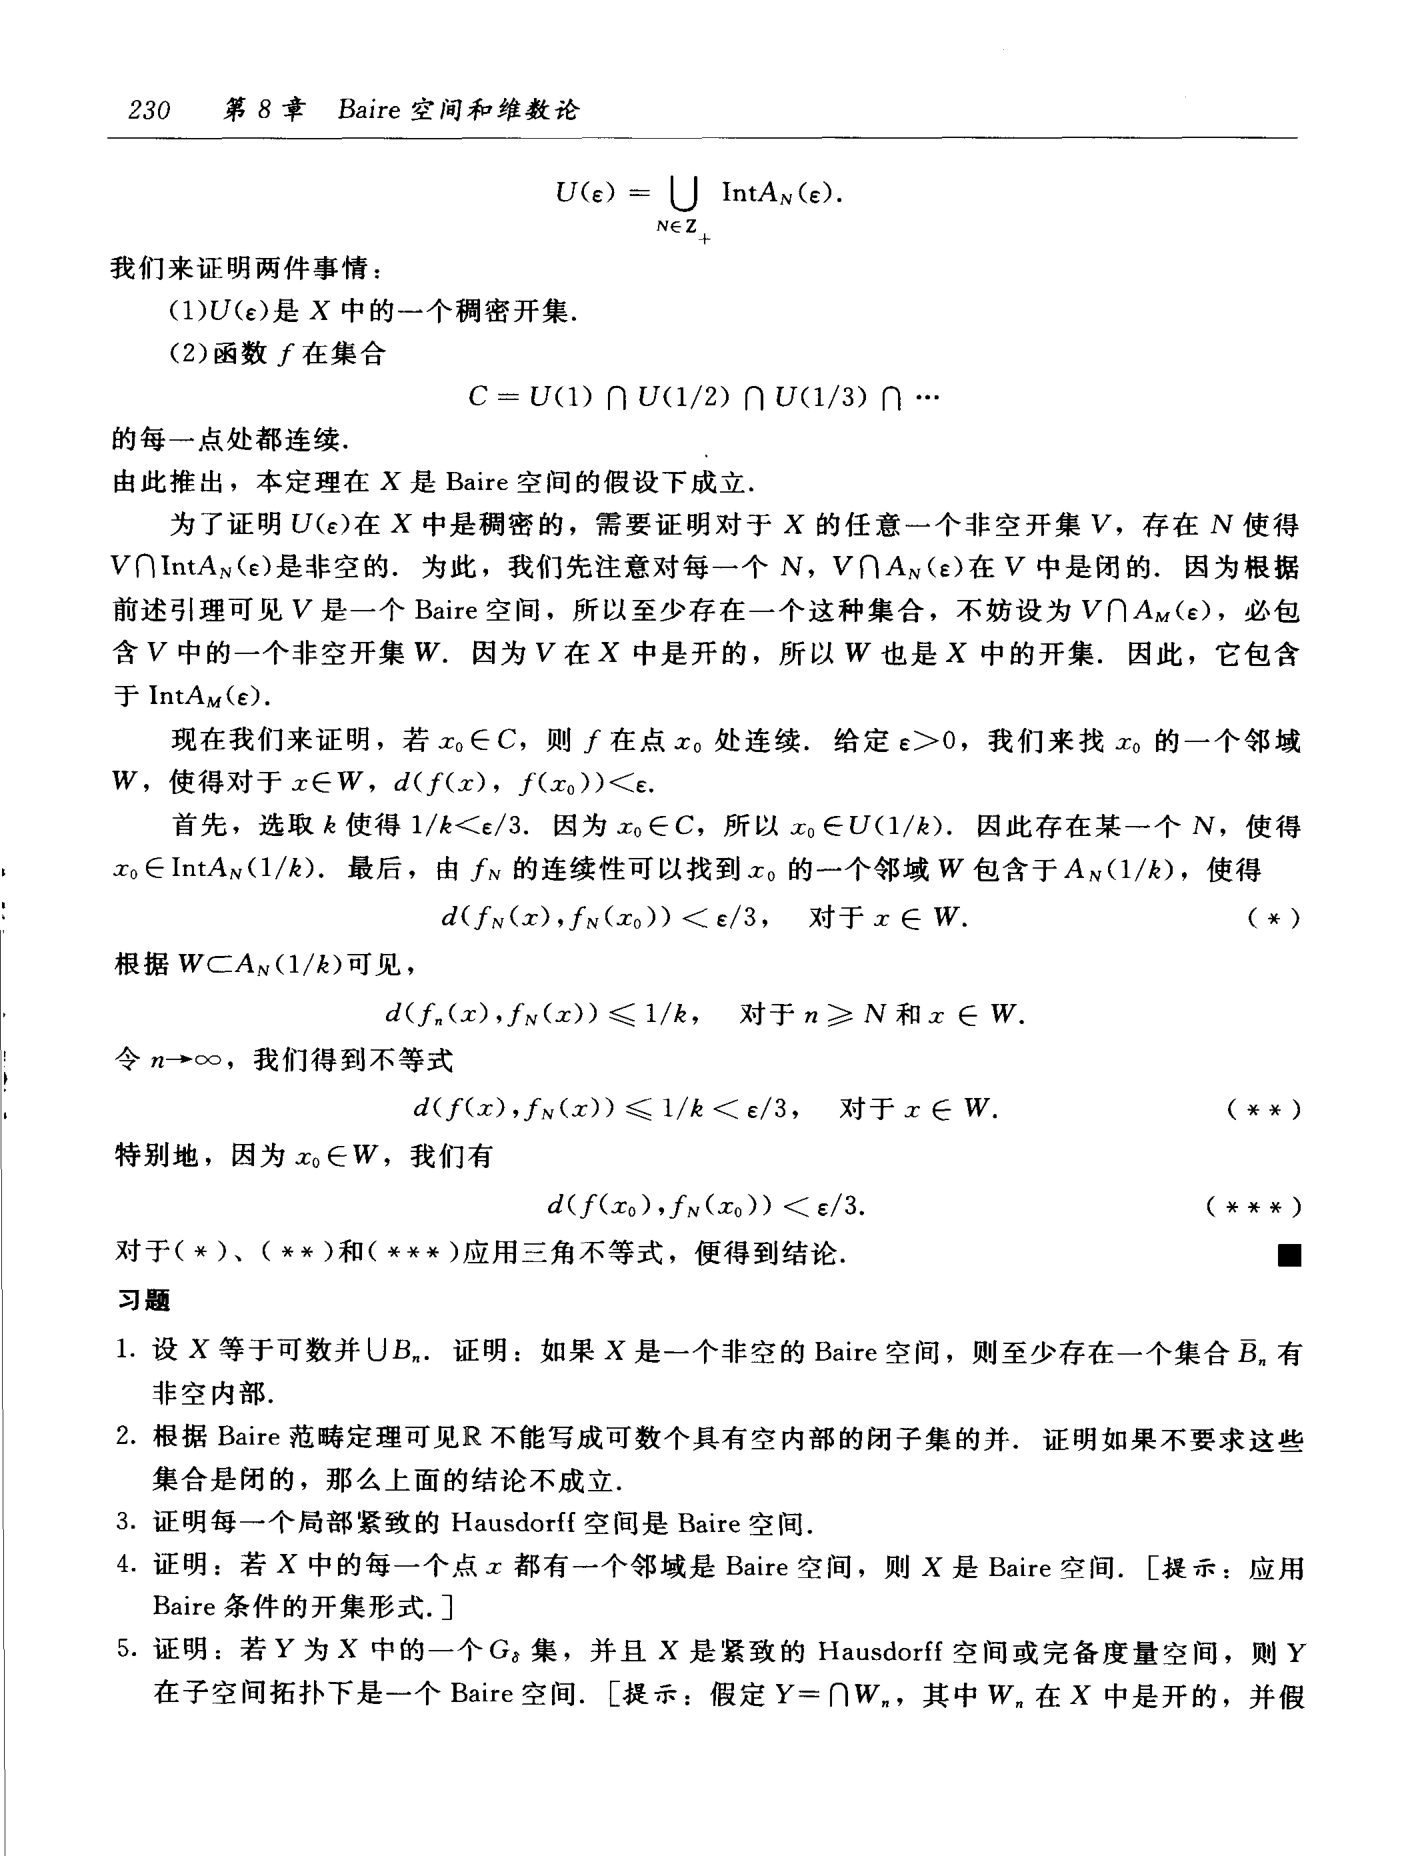
\includegraphics[width=0.8\textwidth]{image/fig-49-1.png}
\caption{$\Delta f(x,h)$ 的几何意义.}
\label{figure:ch08-fig-49-1}
\end{figure}

现在证明关于集合 $U_n$ 的以下结论:

\begin{enumerate}
\item $\bigcap U_n$ 由无处可微函数构成. 设 $f\in\bigcap U_n$, 下面证明对给定的 $x\in[0,1]$, 极限 $\lim\Delta f(x,h)$ 不存在. 给定 $n$, 根据 $f\in U_n$ 可见, 存在一个数 $h_n$, $0<h_n\leqslant 1/n$, 使得
\[
\Delta f(x,h_{n})>n.
\]
因此序列 $(h_n)$ 收敛到 $0$, 但序列 $(\Delta f(x,h_n))$ 不收敛. 因此, $f$ 在点 $x$ 处不可微.

\item $U_n$ 在 $\mathcal{C}$ 中是开的. 设 $f\in U_n$, 我们找 $f$ 的一个 $\delta$-邻域, 使得它包含在 $U_n$ 中. 因为 $f\in U_n$, 故存在 $h$, $0<h\leqslant 1/n$, 使得 $\Delta_h f>n$. 令 $M=\Delta_h f$, 设
\[
\delta=h(M-n)/4.
\]
我们断言, 若 $g$ 是一个满足 $\rho(f,g)<\delta$ 的函数, 则对于所有的 $x\in I$, 有
\[
\Delta g(x,h)\geqslant\frac{1}{2}(M+n)>n,
\]
从而 $g\in U_n$.

为了证明上述论断, 我们先假设 $\Delta f(x,h)$ 等于商 $|f(x+h)-f(x)|/h$. 计算
\[
\left|\frac{f(x+h)-f(x)}{h}-\frac{g(x+h)-g(x)}{h}\right|
=(1/h)\,|\,[f(x+h)-g(x+h)]-[f(x)-g(x)]\,|\leqslant 2\delta/h=(M-n)/2.
\]
如果第一个差商的绝对值至少为 $M$, 那么第二个差商的绝对值至少为
\[
M-\frac{1}{2}(M-n)=\frac{1}{2}(M+n).
\]
若 $\Delta f(x,h)$ 等于另一个差商, 可做相似的讨论.

\item $U_n$ 在 $\mathcal{C}$ 中稠密. 我们需要证明, 对于 $\mathcal{C}$ 中给定的 $f$、给定的 $\varepsilon>0$ 以及给定的 $n$, 可以找到 $U_n$ 中的一个元素 $g$, 使它包含于 $f$ 的 $\varepsilon$-邻域中.

选取 $\alpha>n$, 我们将把 $g$ 构造为一个"分段线性"函数, 也就是说, $g$ 的图像由一条折线组成, 其中 $g$ 的图形中的每一条线段的斜率的绝对值不小于 $\alpha$. 由此立即得出函数 $g$ 属于 $U_n$. 因为令
\[
0=x_{0}<x_{1}<x_{2}<\cdots<x_{k}=1
\]
是区间 $[0,1]$ 的一个分拆, 使得 $g$ 在每一个子区间 $I_i=[x_{i-1},x_i]$ 上的限制是一个线性函数. 再选择 $h$, 使得 $h\leqslant 1/n$ 并且
\[
h\leqslant\frac{1}{2}\min\{\,|x_{i}-x_{i-1}|\,;\ i=1,\cdots,k\,\}.
\]
如果 $x$ 在 $[0,1]$ 中, 则 $x$ 必属于某一个子区间 $I_i$. 如果 $x$ 属于子区间 $I_i$ 的前半段, 则 $x+h$ 也属于 $I_i$, 并且 $(g(x+h)-g(x))/h$ 等于线性函数 $g|I_i$ 的斜率. 类似地, 如果 $x$ 属于子区间 $I_i$ 的后半段, 那么 $x-h$ 属于 $I_i$, 并且 $(g(x-h)-g(x))/(-h)$ 等于线性函数 $g|I_i$ 的斜率. 无论在哪一种情况下, 总有 $\Delta g(x,h)\geqslant\alpha$, 从而 $g\in U_n$.

现在给定 $f$, $\varepsilon$ 和 $\alpha$, 下面说明如何构造上述分段线性函数 $g$. 首先, 由 $f$ 的一致连续性, 选择区间的一个分拆
\[
0=t_{0}<t_{1}<\cdots<t_{m}=1
\]
使得 $f$ 在这个分拆中的每一个子区间 $[t_{i-1},t_i]$ 上的变化最多为 $\varepsilon/4$. 对于每一个 $i=1,\cdots,m$, 选取一点 $a_i\in(t_{i-1},t_i)$, 然后定义一个分段线性函数 $g_1$ 为
\[
g_{1}(x)=
\begin{cases}
f(t_{i-1}) & \text{如果 }x\in[t_{i-1},a_{i}]\\
f(t_{i-1})+m_{i}(x-a_{i}) & \text{如果 }x\in[a_{i},t_{i}],
\end{cases}
\]
其中 $m_i=(f(t_i)-f(t_{i-1}))/(t_i-a_i)$. $f$ 和 $g_1$ 的图像如图 \cref{figure:ch08-fig-49-2} 所示.
\end{enumerate}

\par
\begin{figure}[htbp]
\centering
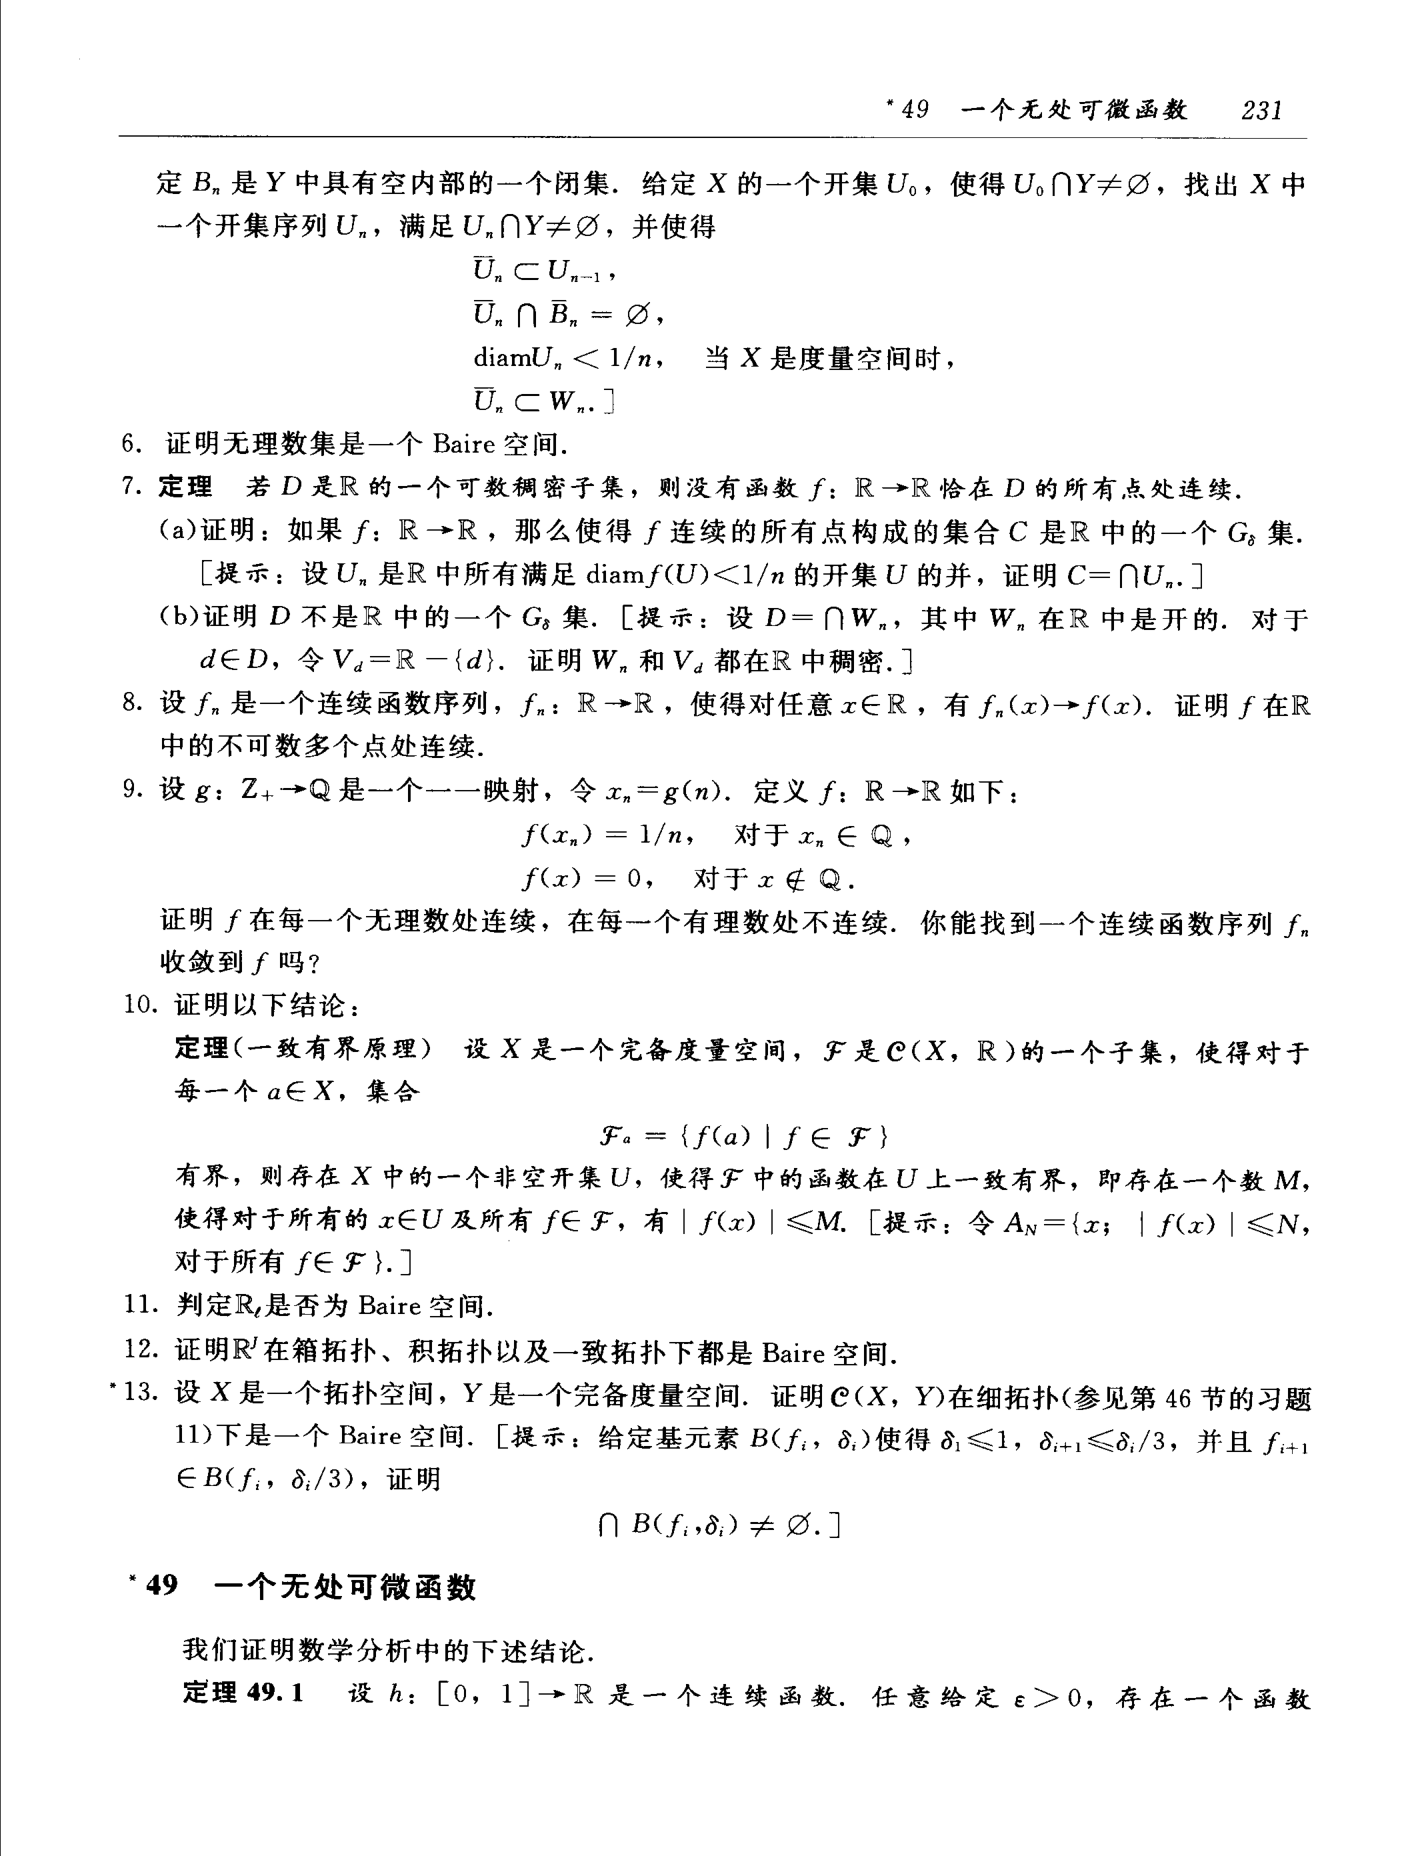
\includegraphics[width=0.8\textwidth]{image/fig-49-2.png}
\caption{$g_1$ 的构造.}
\label{figure:ch08-fig-49-2}
\end{figure}

对点 $a_i$ 的选取要自由些. 如果 $f(t_i)\neq f(t_{i-1})$, 那么我们可以要求 $a_i$ 充分靠近 $t_i$, 使得
\[
t_{i}-a_{i}<\frac{|f(t_{i})-f(t_{i-1})|}{\alpha}.
\]
于是 $g_1$ 的图像将完全由一些斜率为零和斜率的绝对值至少为 $\alpha$ 的线段组成.

进而, 我们断言 $\rho(g_1,f)\leqslant\varepsilon/2$. 这是因为在区间 $I_i$ 上, $g_1(x)$ 与 $f(x)$ 两者相对于 $f(t_{i-1})$ 的变化都不超过 $\varepsilon/4$. 因此, 它们中的每一个相对于另一个的变化不超过 $\varepsilon/2$. 于是, $\rho(g_1,f)=\max\{\,|g_1(x)-f(x)|\,\}\leqslant\varepsilon/2$.

函数 $g_1$ 还不是我们要找的. 现在定义函数 $g$ 如下: 用一个"锯齿形"图像代替 $g_1$ 图像中的水平线段, 并且这些锯齿形全部包含在 $g_1$ 图像的 $\varepsilon/2$ 范围以内, 锯齿的每一条边的斜率的绝对值至少为 $\alpha$. 我们把具体的做法留给读者去完成. 这样, 我们就得到了所要求的函数 $g$. 如图 \cref{figure:ch08-fig-49-3} 所示.

\par
\begin{figure}[htbp]
\centering
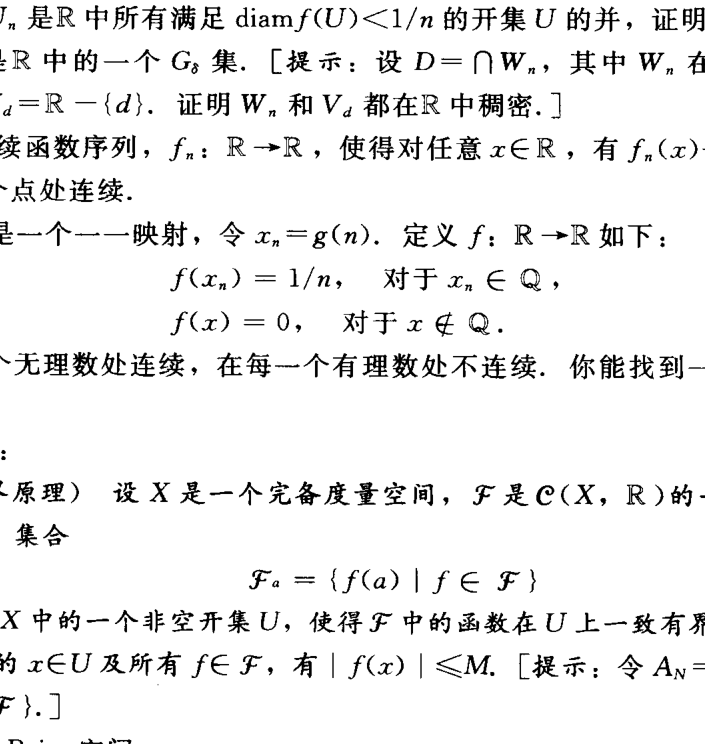
\includegraphics[width=0.8\textwidth]{image/fig-49-3.png}
\caption{锯齿形逼近.}
\label{figure:ch08-fig-49-3}
\end{figure}

\begin{remark}
读者可能会觉得这个证明障碍重重, 似乎过于玄妙而缺乏建设性. 但是, 这个证明中却隐含着一个构造特殊的分段线性函数序列 $f_n$, 使其一致收敛于无处可微函数 $f$ 的过程. 用这种方法定义函数 $f$, 恰好就像通常用无穷级数的极限来定义正弦函数一样是建设性的.
\end{remark}
